
\documentclass[sigconf]{aamas}  % do not change this line!

%% your usepackages here, for example:
\usepackage{booktabs}
\usepackage{enumitem}
\usepackage{balance} 
%\usepackage{microtype}
\usepackage[linesnumbered,vlined,ruled]{algorithm2e}
\newcommand{\todo}[1]{{\color{red} [[TODO: {#1}]]}}
\newcommand{\question}[1]{{\color{blue} [[Question: {#1}]]}}
\newcommand{\dan}[1]{{\color{blue} [[Dan: {#1}]]}}

%% do not change the following lines
%% do not change the following lines
\setcopyright{ifaamas}  % do not change this line!
\acmDOI{}  % do not change this line!
\acmISBN{}  % do not change this line!
\acmConference[AAMAS'18]{Proc.\@ of the 17th International Conference on Autonomous Agents and Multiagent Systems (AAMAS 2018)}{July 10--15, 2018}{Stockholm, Sweden}{M.~Dastani, G.~Sukthankar, E.~Andr\'{e}, S.~Koenig (eds.)}  % do not change this line!
\acmYear{2018}  % do not change this line!
\copyrightyear{2018}  % do not change this line!
\acmPrice{}  % do not change this line!

%% the rest of your preamble here


%%%%%%%%%%%%%%%%%%%%%%%%%%%%%%%%%%%%%%%%%%%%%%%%%%%%%%%%%%%%%%%%%%%%%%%%%%%%%%%%%%%%%%%%%%%%%%%%%%%%%%%%%

\begin{document}

\title{HIGHLIGHTS: Summarizing Agent Behavior to People}  % put your title here!
%\titlenote{Produces the permission block, and copyright information}

% AAMAS: submissions are anonymous for most tracks
%\author{Paper \#148}  % put your paper number here!

%% example of author block for camera ready version of accepted papers: don't use for anonymous submissions
%
\author{Dan Amir}
\affiliation{%
 \institution{The Hebrew University of Jerusalem}
}
\email{dan.amir@mail.huji.ac.il}
\author{Ofra Amir}
\affiliation{%
 \institution{Technion - Israel Institute of Technology}
}
\email{oamir@technion.ac.il}
%\email{trovato@corporation.com}
%


% \author{Lars Th{\o}rv{\"a}ld}
% \authornote{This author is the
%  one who did all the really hard work.}
% \affiliation{%
%  \institution{The Th{\o}rv{\"a}ld Group}
%  \streetaddress{1 Th{\o}rv{\"a}ld Circle}
%  \city{Hekla} 
%  \country{Iceland}}
% \email{larst@affiliation.org}

% \author{Valerie B\'eranger}
% \affiliation{%
%  \institution{Inria Paris-Rocquencourt}
%  \city{Rocquencourt}
%  \country{France}
% }
% \author{Aparna Patel} 
% \affiliation{%
% \institution{Rajiv Gandhi University}
% \streetaddress{Rono-Hills}
% \city{Doimukh} 
% \state{Arunachal Pradesh}
% \country{India}}
% \author{Huifen Chan}
% \affiliation{%
%  \institution{Tsinghua University}
%  \streetaddress{30 Shuangqing Rd}
%  \city{Haidian Qu} 
%  \state{Beijing Shi}
%  \country{China}
% }

% \author{Charles Palmer}
% \affiliation{%
%  \institution{Palmer Research Laboratories}
%  \streetaddress{8600 Datapoint Drive}
%  \city{San Antonio}
%  \state{Texas} 
%  \postcode{78229}}
% \email{cpalmer@prl.com}

% \author{John Smith}
% \affiliation{\institution{The Th{\o}rv{\"a}ld Group}}
% \email{jsmith@affiliation.org}

% \author{Julius P.~Kumquat}
% \affiliation{\institution{The Kumquat Consortium}}
% \email{jpkumquat@consortium.net}
%
%% The example's default list of authors is too long for headers
%\renewcommand{\shortauthors}{B. Trovato et al.}


\begin{abstract}  % put your abstract here!
People increasingly interact with autonomous agents. This paper introduces and formalizes the problem of automatically generating a summary of an agent's behavior with the goal of increasing people's familiarity with the agent's capabilities and limitations. In contrast with prior approaches  which developed methods for explaining a single decision made by an agent, our approach aims to provide users with a summary that describes the agent's behavior in different situations. We hypothesize that reviewing such summaries could help people in tasks such as choosing between agents or determining the level of autonomy to grant to an agent. We develop ``HIGHLIGHTS'', an algorithm that produces a summary of an agent's behavior by extracting important trajectories from simulations of the agent. 
We conducted a human-subject experiment to evaluate whether HIGHLIGHTS summaries help people assess the capabilities of agents. Our results show that participants were more successful at evaluating the capabilities of agents when presented with HIGHLIGHTS summaries compared to baseline summaries, and rated them as more helpful. We also explore a variant of the HIGHLIGHTS algorithm which aims to increase the diversity of states included in the summary, and show that this modification further improves people's ability to assess agents' capabilities.

\end{abstract}



\keywords{Strategy summarization, Explainable AI}  % put your semicolon-separated 
%Explainable AI;Agent-Human Interaction
\maketitle


%%%%%%%%%%%%%%%%%%%%%%%%%%%%%%%%%%%%%%%%%%%%%%%%%%%%%%%%%%%%%%%%%%%%%%%%%%%%%%%%%%%%%%%%%%%%%%%%%%%%%%%%%
%% start of main body of paper

\section{Introduction}
From cleaning robots to self-driving cars, autonomous and semi-autonomous agents are becoming increasingly prevalent~\cite{stone2016artificial}. People's understanding of such agents' behaviors can increase their trust in the agents and their ability to collaborate with them~\cite{devin2016implemented,glass2008toward}. An understanding of an agent's behavior could also support people in tasks such as choosing between alternative agents and determining when the agent can be trusted with performing a task autonomously and when the user's attention is needed. For example, if a user can anticipate the behavior of  a self-driving car in different scenarios, she could be more prepared to take control in situations where the car might not perform well on its own.

While prior work has suggested ways to explain individual decisions of an agent to a person~\cite{khan2009minimal,khan2011automatically}, these approaches do not convey a ``global'' view of an agent's policy. Similarly, recent methods for interpretable machine learning~\cite{vellido2012making,doshi2017towards} typically explain a single decision made by a model, e.g. by presenting a simplified model which justifies decisions in a certain region in the space~\cite{ribeiro2016model}. In this paper, we introduce the problem of providing users with a summary of an agent's behavior. This approach aims to provide users with an overview of the agent's global strategy rather than explaining specific decisions  after the fact. 

A trivial way of communicating an agent's behavior is to show past executions or simulations. This approach, however, has important drawbacks. First, many of the situations an agent encounters might be uninteresting to a person (e.g., a self-driving car stuck in traffic for an hour). Second, reviewing long execution traces will require a person to spend a significant amount of time, and people might give up early, or not pay attention, potentially missing important states. Therefore, we seek solutions that extract \emph{effective} summaries which show the actions taken by the agent in key scenarios. Such summaries can reduce the human effort required to review the agent's behavior, while still providing sufficient information about its capabilities. We note that this is analogous to the approach taken in many settings in which people need to assess the performance of other people. For example, sports scouting agencies typically prepare videos that include highlights from players' games to demonstrate their skills\footnote{e.g.,  \url{https://www.youtube.com/watch?v=gX3e0UM-OeM}. We note that while such scouting videos are often biased to showcase only successful actions, we intend that summaries of agent behavior will include states that demonstrates their behavior in different states of interest, whether successful or not.}.  

%The approach of generating summaries that highlight the capabilities of agents is analogous to other settings in which people need to review the performance of other people. For example, sports scouting agencies prepare videos that include highlights from players' games to demonstrate their skills.\footnote{e.g.,  \url{https://www.youtube.com/watch?v=gX3e0UM-OeM}.}

We developed ``HIGHLIGHTS'', an algorithm that extracts important states from an execution trace of an agent in an online manner. Intuitively, a state is important if different actions in that states can lead to substantially different outcomes for the agent. For example, deciding which turn to take when driving in a city will not be considered important if taking the next turn will result in a similar arrival time; deciding whether to exit a highway will be considered more important, as missing the exit can result in a significant delay. Our approach assumes that HIGHLIGHTS has access to the agent's strategy which is described using a  Markov Decision Process (MDP) policy, and quantifies the importance of states based on the agent's Q-values. To provide more context to the user, rather than showing important states in isolation, the algorithm extracts a trajectory that includes neighboring states and composes a summary of the agent's behavior from these trajectories.

We used HIGHLIGHTS to create summaries of agents playing Mrs. Pacman~\cite{rohlfshagen2011ms} and evaluated these summaries in a human-subject experiment. We compared HIGHLIGHTS summaries with two baselines. One baseline generated summaries by extracting random trajectories of the agent, which will, on average, include states that are more likely to be encountered. The other baseline generated summaries by extracting the first trajectories the agent encountered, which is akin to having a user watch the agent until she runs out of time. In the experiment, participants were shown summaries of different Pacman agents which varied in their performance, and were asked to select an agent to play on their behalf.  They were also asked to rate the helpfulness of different summaries for evaluating an agent's capabilities. 
%They were also shown pairs of summaries of the \emph{same} Pacman agent and were asked to subjectively assess how helpful each of the summaries is for understanding that agent's capabilities. 
Our results show that HIGHLIGHTS led to improved objective performance of participants: they were significantly more likely to choose the better performing agent when the HIGHLIGHTS summaries were shown. HIGHLIGHTS summaries were also rated as more helpful by the study participants. 

%can be condensed to two sentences if needed
One limitation of the HIGHLIGHTS algorithm is that it does not consider the diversity of states in the summary, and therefore if important states are similar to each other, the summary will consist of similar trajectories, thus conveying less new information to users. To mitigate this problem, we developed a variant of the HIGHLIGHTS algorithm which, in addition to state importance, takes into consideration the similarity of the state to other states in the summary. This extension further improved participants' ability to assess the performance of different agents.

The contributions of the paper are threefold: (1) we introduce and formalize the problem of summarizing an agent's behavior to people; (2) we develop HIGHLIGHTS and HIGHLIGHTS-DIV, algorithms that automatically extract summaries of an agent's policy, and (3) we conduct human-subject experiments, showing that summaries generated by HIGHLIGHTS and HIGHLIGHTS-DIV were preferred by participants and improved their ability to assess the capabilities of agents compared to the baseline summaries.

\section{Background \& Related Work\label{sec:related}}

\subsection{Algorithmic Accountability}
As algorithmic approaches replace and supplant human decisions across society, researchers have pointed out the importance of holding algorithms accountable \citep{Gillespie2014,Diakopoulos2015,Garfinkel2017}. One way to do this is the ``algorithm audit,'' which derives its name and approach from longstanding methods in the social sciences designed to detect discrimination \citep{Sandvig2014}. For example, algorithm audits have exposed discrimination in image search algorithms \citep{Kay}, Google auto-complete \citep{Baker2013}, dynamic pricing algorithms \citep{Chen2016}, automated facial analysis \citep{Buolamwini2018}, and word embeddings \citep{Caliskan2017}. Of particular relevance to our work are audit studies focusing on news intermediaries which aggregate, filter, and sort news content from primary publishers.

\subsection{Auditing Intermediaries}
Examples of algorithmic news intermediaries include social media websites (e.g. Facebook, Twitter, reddit), search engines (e.g. Google, Bing), and news aggregation websites (e.g. Google News). On each of these platforms, algorithms select and sort content for millions of users, thus wielding significant power as algorithmic gatekeepers. This content moderation has attracted critical attention \citep{Gillespie2018}, and spurred some researchers to audit intermediaries and check for discrimination, diversity, or filter-bubble effects.

\subsubsection{Social Media}
In the case of social media, \citet{Bakshy} investigated Facebook's News Feed, finding that user choices (e.g., click history, visit frequency) played a stronger role than News Feed's algorithmic ranking when it came to helping users encounter ideologically cross-cutting content. A 2009 study of Twitter showed that trending topics were more than 85\% news-oriented \citep{Kwak2010}. However, because of the high churn rate, trending topics can exhibit temporal coverage bias depending on when users visit the site \citep{Chakraborty2015}.

\subsubsection{Web Search}
As the most popular platform for online search, Google has been the subject of numerous audit studies, some of which reveal discriminatory results. For example, Google's autocomplete feature was shown to exhibit gender and racial biases \citep{Baker2013}, and its image search was shown to systematically underrepresent women \citep{Kay}. Other audits show that user-generated content such as Stack Overflow, Reddit, and particularly Wikipedia play a critical role in Google's ability to satisfy search queries \cite{Vincent2019}

Several studies have investigated potential political bias in Google's search results \citep{Robertson2018,Diakopoulos,Epstein2017}, however, further research is needed to understand the extent and causes of apparent biases. For example, Google's search algorithms may increase exposure to particular news sources (with left-leaning audiences) due to freshness, relevance, or greater overall abundance of content on the web \citep{Trielli}.

Some studies have also investigated Google for creating virtual echo chambers, which may affect democratic processes. While concern has mounted over the search engine's filter-bubble effects \citep{Pariser}, studies have thus far found limited supporting evidence for the phenomenon \citep{Puschmann2018,Flaxman,Hannak2013,Robertson2018}. An analysis of more than 50,000 online users in the United States showed that the search engine can actually ``increase an individual's exposure to material from his or her less preferred side of the political spectrum'' \citep{Flaxman}. Still, some search results may vary with respect to location \citep{Kliman-Silver2015}, an effect that has the potential to create geolocal filter bubbles. %\citep{Hannak2017} examine 200 Google webs earch users and show that ``on average, 11.7\% of results show differences due to personalization.'' Similarly, \citep{Robertson2018} found minimal evidence for the filter bubble hypothesis.

\subsubsection{Google News}
As early as 2005, researchers zeroed in on Google's news system to assess potential bias in the platform \citep{Ulken2005,Schroeder2005}, showing that even shortly after its introduction, scholars were troubled by the platform's potential effects on journalism and the public at large. For example, the Associated Press was concerned that Google used their content without providing compensation \citep{Gaither2005}, and early on, Google News was suspected to have a conservative bias \citep{Ulken2005}.

Google News still attracts critical attention more than a decade later, but concerns have shifted towards the possibility of filter bubbles (as was the case with Google's search engine). Two studies in particular have addressed such concerns: \citet{Haim2018} tested for personalization with manually-created user profiles, and \citet{Nechushtai2019} did so with real-world users. The former study discovered ``minor effects'' on content diversity from both explicit personalization (from user-stated preferences) and implicit personalization (using inferences from observed online behavior). \citet{Nechushtai2019} showed that users with different political leanings and locations ``were recommended very similar news,'' but their study presented a separate concern: just five news outlets accounted for 49\% of the 1,653 recommended news stories. This source concentration highlights the multifaceted implications of news aggregators, which we return to later.


\subsubsection{Apple News}
Apple News has begun to attract the interest of various stakeholders in industry and research. The New York Times wrote about the app in October 2018 \citep{Nicas2018}, focusing on Apple's ``radical approach'' of using humans to curate content instead of just algorithms. Despite its growth, monetization on the platform has thus far proven difficult and drawn criticism \citep{Davies2017,Dotan2018}. Slate reports that it takes 6 million page views in the Apple News app to generate the same advertising revenue as 50,000 page views on its website -- a more than hundredfold difference \citep{Oremus2018}.

A study of Apple News' editorial curation choices in June 2018 analyzed tweets and email newsletters from the editors, finding that larger publishers appeared far more often \citep{Brown2018}. In a followup study, screen recordings captured the Top Stories section in the United Kingdom to collect 1,031 total articles, 75\% of which came from just six publishers \citep{Brown2018a}. This paper builds on and adds to these studies in two important ways. First, we design and use a method for \textit{fully automated data collection}, rather than relying on manual coding of screen recordings. This method allows us to collect both Top Stories and Trending Stories in the United States, whereas \citep{Brown2018a} collected only Top Stories in the United Kingdom. Second, we examine mechanical aspects of Apple News in addition to examining content. By investigating mechanisms such as adaptation and update frequency, we reveal several intriguing design choices and curation patterns within the app.
\section{Summarizing Agent Behaviors}
\label{sec:problem}
%To help people better understand the capabilities of agents, we propose to generate summaries of an agent's behavior. 
%Because in most settings it will not be feasible to describe the agent's behavior in each of the possible states. 
Our formalization of the summarization problem assumes that the agent uses a Markov Decision Process (MDP), where $A$ is the set of actions available to the agent, $S$ is the set of states, $R$: $S \times A \rightarrow \mathbb{R}$ is the reward function, which maps each state and action to a reward, and $Tr$ is the transition probability function, i.e., $Tr(s', a, s)$ defines the probability of reaching state $s'$, when taking action $a$ in state $s$. The agent has a policy $\pi$ which specifies which action to take in each of the states. 

We formalize the problem of summarizing an agent's behavior as follows: from execution traces of an agent, choose a set $T = \langle t_{1},...,t_{k} \rangle$ of trajectories to include in the summary, where each trajectory is composed of a sequence of $l$ consecutive states and the actions taken in those states $\langle(s_{i},a_{i}),...,(s_{i+l-1},a_{i+l-1})\rangle$. We consider trajectories rather than single states because seeing what action was taken by the agent in a specific state might not be meaningful without a broader context (e.g., watching a self-driving car for one second will not reveal much useful information). Because it is infeasible that people will be able to review the behavior of an agent in all possible states, we assume a limited budget $k$ for the size of the summary, such that $|T| = k$. This budget limits the amount of time and cognitive effort that a person needs to invest in reviewing the agent's behavior. We discuss alternative formulations of the summarization problem in Section~\ref{sec:disc}. 

There are several factors that could be considered when deciding which states to include in a summary, such as the effect of taking a different action in that state, the diversity of the states that are included in the summary and the frequency at which states are likely to be encountered by the agent. In this paper, we focus on the first factor, which we refer to as the ``importance'' of a state. Intuitively, a good summary should provide a person reviewing the summary with a sense of the agent's behavior in states that the person considers important (e.g., when making a mistake would be very costly). The importance of states included in the summary could substantially affect the ability of a person to assess an agent's capabilities. For example, imagine a summary of self-driving car that only shows the car driving on a highway with no interruptions. This summary would provide people with very little understanding of how the car might act in other, more important, scenarios (e.g., when another car drives into its lane, when there is road construction). In contrast, a summary showing the self-driving car in a range on more interesting situations (e.g., overtaking another car, breaking when a person enters the road) would convey more useful information to people reviewing it. 

In Section~\ref{sec:alg} we describe an algorithm that generates summaries based on this state importance criteria. We then extend the algorithm to also take into consideration the diversity of the states included in the summary (described in Section~\ref{sec:algDiv}). That is, instead of considering each state in isolation when deciding whether to include it in the summary, the decision will also depend on the other states that are currently included in the summary. We discuss other possible desired summary properties in Section~\ref{sec:disc}. 

%Intuitively, a good summary should provide a person reviewing the summary with a sense of the agent's behavior in states that the person considers important (e.g., when making a mistake would be very costly). The choice of trajectories to include in the summary could substantially affect the ability of a person to assess an agent's capabilities. For example, imagine a summary of self-driving car that only shows the car driving on a highway with no interruptions. Such summary would provide people with very little understanding of how the car might act in other scenarios (e.g., when another car drives into its lane, when there is road construction). In contrast, a summary showing the self-driving car in a range on more interesting situations would likely convey more useful information to people reviewing it. 

%Second, we might want to produce a summary that is diverse, in the sense that it describes the behavior of the agent in a scenarios that differ from one another. 

\section{The ``Highlights'' Algorithm}
\label{sec:alg}
We developed HIGHLIGHTS, an algorithm that generates a summary of an agent's behavior from simulations of the agent in an online manner. HIGHLIGHTS uses the notion of state \emph{importance}~\cite{torrey2013teaching} to decide which states to include in the summary.  Intuitively, a state is considered important if taking a wrong action in that state can lead to a significant decrease in future rewards, as determined by the agent's Q-values. Formally, the importance of a state, denoted $I(s)$, is defined as: 
\begin{equation}
\label{eq:importance}
I(s)=\max\limits_{a}Q^{\pi}_{(s,a)}-\min\limits_{a}Q^{\pi}_{(s,a)}
\vspace{-0.1cm}
\end{equation}
 This measure has been shown to be useful for choosing teaching opportunities in the context of student-teacher reinforcement learning~\cite{torrey2013teaching,amirIjcaiRL}. We note, however, that this measure has significant limitations (e.g., sensitivity to the number of possible actions) which we discuss in Section~\ref{sec:disc}.

Before providing a detailed pseudo-code of the algorithm, we describe its operation at a high-level. HIGHLIGHTS generates a summary that includes trajectories that captures the most important states that an agent encountered in a given number of simulations. To do so, at each step it evaluates the importance of the state and adds it to the summary if its importance value is greater than the minimal value currently represented in the summary (replacing the minimal importance state). To provide more context to the user,  for each such state HIGHLIGHTS also extracts a trajectory of states neighboring it and the actions taken in those states.

%To do so, the algorithm runs simulations of the agent and maintains a priority queue of trajectories  to include in the summary. For each state $s$ the agent encounters, HIGHLIGHTS evaluates the state importance as defined in Equation~\ref{eq:importance}. If the importance of the state is greater than the minimal importance of a state that is currently included in the summary, that state will be removed and replaced with the current state $s$. Because a single state is non-informative on its own in many domains, rather than only including $s$ in the summary, HIGHLIGHTS considering a trajectory of length $l$ that includes $s$ (showing both states preceding $s$ and subsequent states). At the end of this process, the summary will include trajectories corresponding to the most important states the agent encountered in the simulation\footnote{In this work we choose trajectories for the summary based on the importance of a single state in the trajectory. We discuss possible extensions that assess the importance of a complete trajectory in Section~\ref{sec:disc}.}). To avoid including overlapping trajectories, we enforce an interval between trajectories (i.e., we do not consider states that appear immediately after a trajectory that was added to the summary). 

%The algorithm runs simulations of the agent and extracts states that it considers important, using the basic q-value-based importance defined in Equation~\ref{eq:importance}. It maintains a priority queue of size $k$ and populates it online while running the agent simulation. Specifically, when a new state $s$ is encountered and the queue is not yet full, the state is added to the queue. Alternatively, if the queue is full, the importance value of the state ($I(s)$) is compared with the lowest importance value currently in the queue. If $I(s)$ is greater than $I(s_{min})$, state $s$ will be added to the queue in place of $s_{min}$. To provide context in the summary, for each state we also show a trajectory of $\frac{l}{2}$ states which preceded $s$ in the execution and the $\frac{l}{2}$ states encountered following $s$. To ensure that trajectories do not overlap, after adding a trajectory to the summary we assess the state immediately following the last state in the trajectory.

A pseudo-code of the HIGHLIGHTS algorithm is  given in Algorithm~\ref{alg:highlights}. 
Table~\ref{tb:parameters} summarizes the parameters of the algorithm. 
HIGHLIGHTS takes as input the policy of the agent $\pi$ which is used to determine the agent's actions in the simulation and state importance values, the budget for the number of trajectories to include in the summary ($k$) and the length of each trajectory surrounding a state ($l$). Each such trajectory includes both states preceding  the important state and states that were encountered immediately after it. The number of subsequent states to include is determined by the $statesAfter$ parameter (the number of preceding states can be derived from this parameter and $l$). We also specify the number of simulations that can be run ($numSimulations$), and the minimal ``break'' interval between trajectories ($intervalSize$) which is used to prevent overlaps between trajectories. HIGHLIGHTS outputs a summary of the agent's behavior, which is a set of trajectories ($T$). 


\begin{table}[h]
\centering
\small
\resizebox{0.85\columnwidth}{!}{%
\begin{tabular}{|p{2.2cm}|p{6cm}|}
\hline
\textbf{Parameter} & \textbf{Description (value used in experiments)}                      \\ \hline
$k$                & Summary budget, i.e., number of trajectories (5)                                  \\ \hline
$l$                & Length of each trajectory (40)                                        \\ \hline
$numSimulations$   & The number of simulations run by HIGHLIGHTS (50)                      \\ \hline
$intervalSize$     & Minimal number of states between two trajectories in the summary (50) \\ \hline
$statesAfter$      & Number of states following $s$ to include in the trajectory (10)      \\ \hline
\end{tabular}}
\caption{Parameters of the HIGHLIGHTS algorithm and the values assigned to them in the experiments (in parentheses).}
\label{tb:parameters}
\vspace{-0.7cm}
\end{table}

% \begin{table}[h]
% \centering
% \small
% \begin{tabular}{|p{2.1cm}|p{3.8cm}|p{1.7cm}|}
% \hline
% \textbf{Parameter} & \textbf{Description}                                         & \textbf{Value in \hspace{2em} Experiments} \\ \hline
% $k$                & Summary budget (\# trajectories)                             & 5                             \\ \hline
% $l$                & Length of each trajectory                                    & 40                            \\ \hline
% $numSimulations$   & The number of simulations run by HIGHLIGHTS                  & 50                            \\ \hline
% $intervalSize$     & Minimal number of states between two trajectories & 50                            \\ \hline
% $statesAfter$      & Number of states following $s$ to include in the trajectory      & 10                            \\ \hline
% \end{tabular}
% \caption{Parameters of the HIGHLIGHTS algorithm and the values assigned to them in the experiments.}
% \label{tb:parameters}
% \vspace{-0.3cm}
% \end{table}

The algorithm maintains two data structures: $T$ is a priority queue (line 2), which will eventually hold the trajectories chosen for the summary; $t$ is a list of state-action pairs (line 3), which holds the current trajectory the agent encounters. The procedure runs simulations of the agent acting in the domain. At each step of the simulation, the agent takes an action based on its policy and advances to a new state (line 8). That state-action pair is added to the current trajectory (line 11). If the current trajectory reached its maximal length, the oldest state in the trajectory is removed (lines 9-10).  HIGHLIGHTS computes the importance of $s$ based on the Q-values of the agent itself, as defined in Equation~\ref{eq:importance} (line 14). 

If a sufficient number of states were encountered since the last trajectory was added to the summary, state $s$ will be considered for the summary (the $c==0$ condition in line 17). $s$ will be added to the summary if one of two conditions hold: either the size of the current summary is smaller than the summary size budget, or the importance of $s$ is greater than the minimal importance value of a state currently represented in the summary (line 17). If one of these conditions holds, a trajectory corresponding to $s$ will be added to the summary. The representation of a trajectory in the summary (a $summaryTrajectory$ object) consists of the set of state-action pairs in the trajectory (which will be presented in the summary), and the importance value $I_{s}$ based on which the trajectory was added (such that it could be compared with the importance of states encountered later). This object ($st$) is initialized with the importance value (line 20) and is added to the summary (line 21), replacing the trajectory with minimal importance if the summary reached the budget limit (lines 18-19).
%For each such state, we store the importance value based on which it was added to the summary and the trajectory of states surrounding it. 
%replacing the trajectory with minimal importance if the summary already reached the budget limit (lines 18-19). For each trajectory we store the state based on which it was added (line 20), such that we can compare its importance to new states as they are encountered. 
%If one of these conditions holds, a trajectory corresponding to $s$ will be added to the summary (line 21), replacing the trajectory with minimal importance if the summary already reached the budget limit (lines 18-19). For each trajectory we store the state based on which it was added (line 20), such that we can compare its importance to new states as they are encountered. 
Because the trajectory will also include states that follow $s$, the final set of state-action pairs in the trajectory is updated later (lines 15-16). Last, we set the state counter $c$ to the interval size, such that the immediate states following $s$ will not be considered for the summary. At the end of each simulation, the number of runs is incremented (line 24). The algorithm terminates when it reaches the specified number of simulations. 

% HIGHLIGHTS considers adding the trajectory corresponding to the current state $s$ unless f a sufficient number of states were encountered since the 

% , adding each state $s$ it encounters to the current trajectory. If the trajectory is at the maximal length, the new state replaces the oldest state in $t$ (lines 6--9). 

% If the summary size has not yet reached the budget, the current trajectory $t$ will be added to the summary (lines 11 --13). Otherwise, the trajectory will be added only if the importance of the last state encountered ($I(s)$) is greater than the minimal importance value currently in the summary (lines 13--15). We note that in our implementation of HIGHLIGHTS, to provide more context surrounding the important state, we added to the trajectory the 10 states that followed $s$ (removing the first 10 states in the trajectory to maintain a trajectory length $l$). We did not include this in the pseudo-code for clarity of presentation. 
% =
\begin{algorithm}
%\vspace{-0.2cm}
\SetAlFnt{\small\sf} 
\DontPrintSemicolon % Some LaTeX compilers require you to use \dontprintsemicolon instead
\KwIn{$\pi, k, l, numSimulations, intervalSize, statesAfter$}
\KwOut{$T$}
$runs = 0$ \\
$T \leftarrow PriorityQueue(k, importanceComparator)$ \\
$t \leftarrow$ empty list \\
$c = 0$ \\
\While {$(runs < numSimulations)$} {
$sim = InitializeSimulation()$ \\
\While {$(!sim.ended())$} {
$(s,a) \leftarrow sim.advanceState(\pi)$ \\
\If{$(|t| == l)$} {
$t.remove()$ 
}
$t.add((s,a))$ \\
\If {$(c>0)$} {
$c = c-1$
}
$I_{s} \leftarrow computeImportance(\pi,s)$ \\
\If{$(IntervalSize - c == statesAfter)$} {
lastSummaryTrajectory.setTrajectory(t) \\
}
% $I_{s} \leftarrow computeImportance(\pi,s)$ \\
% \uIf{$|T|<k$} {
% $T.add(t)$ 
% }
% \ElseIf{$I_{s} > minImportance(T)$} {
% T.pop() \\
% $T.add(t)$ 
% }
\If{($(|T|<k)$ or $(I_{s} > minImportance(T)))$ and $(c==0))$ } {
\If{$|T|==k$} {
T.pop()
}
$st\leftarrow$ new $summaryTrajectory(I_{s})$ \\
$T.add(st)$ \\
$lastSummaryTrajectory \leftarrow st$ \\
$c = intervalSize$ \\
}
}
runs = runs+1
}
\caption{The HIGHLIGHTS algorithm. }
\label{alg:highlights}
\end{algorithm}

%\vspace{-0.5cm}


 We chose to implement HIGHLIGHTS as an online algorithm  because it is less costly, both in terms of runtime and in terms of memory usage. 
 %For example, if important states are rare, it might be too costly to store all the states encountered and analyze them retrospectively. 
 In addition, such an algorithm can be incorporated into the agent's own learning process without additional cost. The algorithm can be easily generalized to work offline. 
 
\subsection{Considering State Diversity}
\label{sec:algDiv}
Because HIGHLIGHTS  considers the importance of states in isolation when deciding whether to add them to the summary, the produced summary might include trajectories that are similar to each other. This could happen in domains in which the most important scenarios tend to be similar to each other. To mitigate this problem, we developed a simple extension to the HIGHLIGHTS algorithm, which we call HIGHLIGHTS-DIV. Similarly to HIGHLIGHTS, this algorithm also determines which states to include in the summary based on their importance. However, it also attempts to avoid including a very similar set of states in the summary, thus potentially utilizing the summary budget more effectively. 

HIGHLIGHTS-DIV takes into consideration the diversity of states in the following way: when evaluating a state $s$, it first identifies the state most similar to $s$ that is currently included in the summary\footnote{We assume that distance metric to compare states can be defined. This can be done in many domains,  e.g., by computing Euclidean distance if states are represented by feature vectors.}, denoted $s'$. Then, instead of comparing the importance of a state to the minimal importance value that is currently included in the summary, HIGHLIGHTS-DIV compares $I_{s}$ to $I_{s'}$. If $I_{s}$ is greater than $I_{s'}$, the trajectory which includes $s'$ in the summary will be replaced with the current trajectory (which includes $s$). This approach allows less important states to remain represented in the summary (because they will not be compared to some of the more important states that differ from them), potentially increasing the diversity of trajectories in the summary and thus conveying more information to users. 






\section{Empirical Methodology}
\label{sec:empirical}
%To evaluate HIGHLIGHTS and HIGHLIGHTS-DIV, we conducted experiments in which participants were shown summaries produced by these algorithms, as well as summaries produced by baseline methods. We next describe the empirical domain used in our experiment, the experimental conditions and the 
\paragraph{Empirical Domain.} To evaluate HIGHLIGHTS and HIGHLIGHTS-DIV, We generated summaries of agents playing the Mrs. Pacman game~\cite{rohlfshagen2011ms}. Figure~\ref{fig:pacman} shows a screen from the experiment which includes snapshots of the Pacman maze used in our experiments. This game configuration includes two types of food pellets: regular pellets (small dots) are worth 10 points each and power pellets (larger dots) are worth 50 points each. After eating a power pellet, ghosts become edible for a limited time period. Pac-Man receives 200 points for each ghost it eats. Ghosts chase Pac-Man with $80\%$ probability and otherwise move randomly. In each state, Pac-Man has at most four moves (right, left, up or down). Important states in the game include situations where Pacman is very close to ghosts (e.g., the state shown for the Pacman game on the right side in Figure~\ref{fig:pacman}) or  when Pacman has an opportunity to eat a power pellet, or a ghost. 

Due to the large size of the state space, we used the high-level 7-feature representation from Torrey \& Taylor's~\shortcite{torrey2013teaching} implementation. Q-values are defined as a weighted function of the feature values, i.e., $Q(s,a)=\omega_{0}+\sum_{i}{\omega_{i} \cdot f_{i}(s,a)}$
% \begin{equation}
% Q(s,a)=\omega_{0}+\sum_{i}{\omega_{i} \cdot f_{i}(s,a)}
% \label{e:q}
% \vspace{-0.3cm}
% \end{equation}  


\begin{figure}[h]
	\centering
    \frame{
	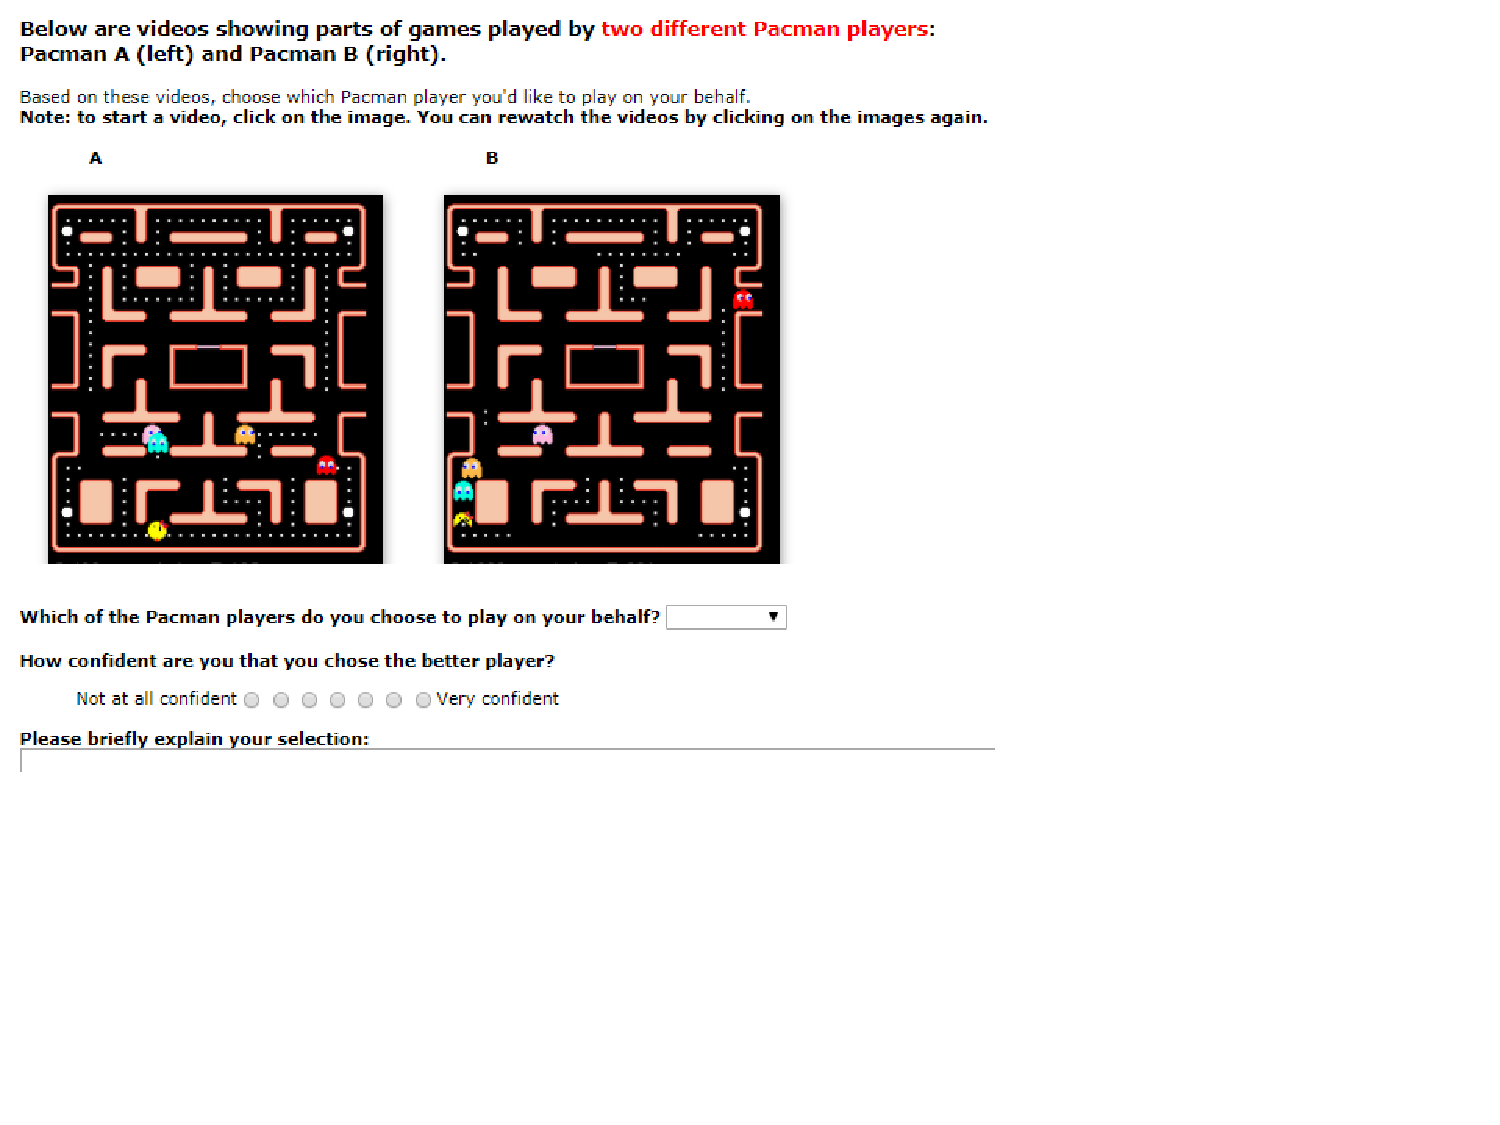
\includegraphics[width=0.98\columnwidth]{figs/pacman.pdf}}\\
	\caption{A screenshot of the agent selection task.}
	\label{fig:pacman}
	\vspace{-0.4cm}
\end{figure}


% \begin{figure}
% 	\centering
% 	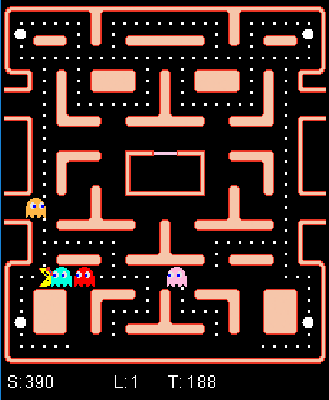
\includegraphics[width=0.3\columnwidth]{figs/pacman1.pdf}\\
% 	\caption{The Mrs. Pac-Man Game.}
% 	\label{fig:pacman}
% 	\vspace{-0.4cm}
% \end{figure}




\paragraph{Experimental Conditions.} In addition to generating summaries using the two versions of the HIGHLIGHTS algorithm, we also generated summaries using two baseline methods:
\begin{itemize}[leftmargin=.3cm]
\item \emph{First}: a summary is generated from the first $k$ trajectories Pacman encounters. This baseline is akin to having a user watch the agent act (e.g., watching a video of an autonomous vehicles driving) until she runs out of time.
\item \emph{Random}: a summary is generated by sampling $k$ trajectories uniformly from the agent's execution trace. %Since we generate the summaries online, we used reservoir sampling~\cite{vitter1985random} which extracts random samples from an online stream. 
With this baseline states that are more frequently encountered are more likely to be selected to the summary. 
\end{itemize}

The parameter values for the algorithms used to generate the Pacman summaries are listed in Table~\ref{tb:parameters}.  All summaries included five trajectories ($k=5$), each showing 40 neighboring states ($l$=40). 
%We used $statesAfter=10$, meaning that each trajectory included 10 states following the important state (the first 29 states were the states preceding the important state). 
They enforced a gap of 50 states before considering a state for inclusion in the summary (i.e., $intervalSize = 50$).  To present the summaries to users, we generated video-clips (GIF files) showing the trajectories that were chosen for the summary\footnote{See example summary video here: \url{https://goo.gl/79dqsd}.}. We note that the summaries shown to participants did not include the current score of the agent (see Figure~\ref{fig:pacman}) to ensure that participants' evaluation will  be based on the observed behavior of the Pacman player rather than its score.

We generated three different agents by varying their training period. The lowest performing agent was trained for 200 episodes (scores 2262 points on average), the medium agent for 400 episodes (scores 2732 points on average), and the highest performing agent was trained for 2000 episodes (scores 3826 points on average). Henceforth, we refer to these agents as the \emph{200E}, \emph{400E} and \emph{2000E} agent, respectively. Generating agents of varying performance enabled us to have a ground truth when asking participants to assess the agents' performance. The summaries were generated after the agents were fully trained and reflect the final policies of the agents.  



%Participants completed two types of task, described in more detail in Section~\ref{sec:procedure}. In the first task, participants were shown summaries of two different agents, and were asked to choose which agent they want to play on their behalf. This task provides an objective way of assessing whether the summaries helped participants assess the performance of different agents. In the second task, participants were shown two summaries of \emph{the same} agent, and were asked which summary they found more helpful for assessing the agent's capabilities. This task provided a subjective measure assessing the perceived usefulness of the summaries. For these tasks, we generated three different agents by varying their training period. The lowest performing agent was trained for 200 episodes, the medium agent for 400 episodes, and the highest performing agent was trained fro 2000 episodes. Henceforth we refer to these agents as the \emph{200E}, \emph{400E} and \emph{2000E} agent, respectively. Generating agents of varying performance enabled us to have a ground truth for the agent selection task. The summaries were generated after the agents were fully trained, such that they reflect the final policies of the agents.  

We conducted two experiments. Experiment 1 compared the HIGHLIGHTS algorithm with the two baseline methods. Experiment 2 compared the HIGHLIGHTS-DIV algorithm with the basic HIGHLIGHTS algorithm and the \emph{Random} baseline. We used the same procedure in both experiments. 

\paragraph{Procedure}
%\label{sec:procedure}
Participants were first shown a tutorial explaining the rules of the Pacman game. They then had to pass a quiz ensuring they read and understood the rules. Next, they were asked to complete two different tasks (described next). Participants received a base payment of \$1.5, and could earn a bonus of up to \$0.9 (explained in task 1). We used a within-subject study design, such that all participants evaluated all summary methods. 
%An anonymized version of the study (without the consent form) can be accessed here ***add url***. 

\textbf{Task 1: Agent Selection.}
In the first task, participants were shown pairs of  summaries of two \emph{different} Pacman agents, produced by the \emph{same} summary method (e.g., a HIGHLIGHTS summary of the \emph{200E} agent and a HIGHLIGHTS summary of the \emph{400E}). They were asked to choose the agent they would like to play on their behalf. Participants were also asked to explain their selection and to rate their confidence in their decision on a 7-point Likert scale (1 - not at all confident to 7 - very confident). Overall, there were 9 such pairs (3 agent levels X 3 summarization methods).  An example agent selection task is shown in Figure~\ref{fig:pacman}. The ordering of pairs to compare as well as which summary was shown on the left and which on the right were randomized. Participants were given a bonus of 10 cents for each correct agent selection, such that they had a monetary incentive to select the better performing agent. 

The different agent comparisons differed in the difficulty of identifying the better agent: the \emph{200E} and \emph{400E} agents had the most similar performance, resulting in a \emph{high-difficulty} comparison; the \emph{200E} and \emph{2000E} agents differed most substantially in their performance, resulting in a \emph{low-difficulty} comparison; we refer to the comparison of  the \emph{400E} and \emph{2000E} agents as the \emph{medium-difficulty} comparison, as the differences in the agents' policies were more substantial than for the \emph{200E} and \emph{400E} agents, but less substantial than for the \emph{200E} and \emph{2000E} agents. 

\textbf{Task 2: Summary Preferences.}
While the first task measured participants' objective ability to identify the better agent, in the second task we elicited participants' subjective opinions about the helpfulness of different summaries. They were again shown pairs of summaries. This time the two summaries were of \emph{the same} agent (participants were told it was the same agent), but were generated by a \emph{different} summary method (e.g., comparing a HIGHLIGHTS summary of the 200E agent with a \emph{Random} summary of the 200E agent). Participants were asked to rate which of the summaries they find more helpful for assessing the capabilities of the Pacman agent using a 7-point Likert scale (1 - video A is more helpful, 7 - video B is more helpful). They were also asked to provide a short explanation for their preference. 

To maintain a reasonable experiment length and because we were primarily interested in the usefulness of HIGHLIGHTS summaries, in this task participants only made 4 comparisons (2 of the 3 agents, comparing HIGHLIGHTS summaries with each of the baseline summaries). The ordering of pairs to compare as well as their location on the screen (left or right) were randomized. 

\paragraph{Evaluation Metrics and Analyses}
The analysis of task 1 evaluated participants' correctness rate when selecting Pacman agents with each summary method. We analyzed the data using a logistic regression, controlling for the comparison type (200E vs. 400E agents, 400E vs. 2000E agents or 200E vs. 2000E agents). Since we used a within-subject design, we ran a repeated measures logistic regression. We also compared participants' confidence in making these selections. Confidence ratings were analyzed using an ordinal logistic regression, again controlling for the comparison type.  For the fitted regression models, we report the significance of the coefficients as well as the odds ratio values ($OR$), which can be interpreted as effect sizes. Values between 1.5 and 3 are interpreted as a small effect, between 3 and 5 as medium, and above 5 as large~\cite{borenstein2009converting,chen2010big}.

When analyzing task 2, we compared the helpfulness ratings given to the summaries. We normalized the preferences such that 7 always means ``HIGHLIGHTS is more helpful'' and 1 means ``[other method] is more helpful''. That is, a rating greater than 4 indicates a preference for HIGHLIGHTS. We analyzed these ratings using the non-parametric Wilcoxon rank sum test.\footnote{We used Wilcoxon rank sum as the scale was ordinal and the data was not normally distributed. However, we obtain similar results when using standard t-test.}

To account for multiple hypotheses testing, we adjusted p-values with the Holm's sequentially rejective Bonferroni procedure~\cite{holm79:simple,shaffer95:multiple}. We report raw p-values, but in all cases we state significant differences, the adjusted p-values were also smaller than $0.05$.





\section{Experiment 1: Basic HIGHLIGHTS}
Experiment 1 compared summaries generated by the basic HIGHLIGHTS algorithm, which only considers state importance, with summaries generated with the \emph{Random} and \emph{First} baselines. 40 participants were recruited through Amazon Mechanical Turk (23 female, Mean age = 35.35, STD = 10.4).  


%\label{sec:exp1res}
\paragraph{Agent Selection Results}
\label{sec:exp1res}
As shown in Figure~\ref{fig:highlightsRes}, participants were more likely to choose the better performing agents when shown summaries generated by the HIGHLIGHTS algorithm compared to the baselines. The analysis shows statistically significant and substantial differences in performance when comparing HIGHLIGHTS to  \emph{First} ($\chi^2=49.79, p<1^{-10}, OR = 12.09$) and when comparing HIGHLIGHTS to \emph{Random} ($\chi^2=6.93, p=0.001, OR = 2.38$). 

When comparing HIGHLIGHTS and \emph{First}, we found a  significant difference for all three agent comparison types (low, medium and high difficulty). When comparing HIGHLIGHTS to \emph{Random}, we observed a significant difference only for the \emph{medium-difficulty} comparison (\emph{400E} vs. \emph{2000E} agents). This makes sense as the difference between the \emph{200E} and \emph{400E} agents is relatively small, making the comparison hard with any summary. The difference between the \emph{200E} vs. \emph{2000E} agents is very substantial, making it easier to identify the better agent even with random trajectories. Interestingly, for the low-difficulty comparison, the summaries generated by \emph{First} were particularly misleading. We hypothesize the reason for this is that participants saw the \emph{2000E} agent taking more risks initially, as participants' explanations often referred to the \emph{2000E} agent behavior as risky, e.g. ``Player B [2000E] made some risky turns which will end his play before Player A [200E].'' 

We observed different types of explanations provided by participants. Some explanations referred directly to the capabilities demonstrated by the agent in the summary, e.g. ``B [2000E] seems like they are better at actually eating the ghosts''. Other participants noted the state of the board shown in different summaries, e.g. ``B has more of the screen cleared''. Some explanations described the general behavior of the agent, e.g. ``Pacman B seems to be effective at routing'' or how Pacman's strategy compares to their own strategy, e.g. ``He went the way I would have.'' Last, some explanations referred to specific events, e.g. ``Pacman a looked like it was about to be cornered.'' 

The type of explanation provided often depended on the summary method used and the difficulty of the agent comparison. Participants' explanations when shown HIGHLIGHTS summaries for the low-difficulty and medium-difficulty comparisons typically referred to specific capabilities they observed, e.g. ``Player A [2000E] is eating ghost so earning more points.'' We observed fewer such explanations for the high-difficulty comparison, e.g. ``Player B has eaten one power pill which means he's had the chance to go after the ghosts (for more points) at least once.  Also seems to have eaten more dots on the whole than Player A.'' Explanations for this comparison more often pointed to the state of the board or provided a general impression of the agent's behavior.
%Other explanations referred to the state of the board shown in the trajectories, e.g. ``B has more of the screen cleared'', or provided a general impression of the agent's behavior, e.g. ``Pacman B seems to be effective at routing''. 
For the \emph{First} summaries, participants typically conveyed their general impression of the agent's behavior. Explanations for the \emph{Random} baseline were similar to those given in the HIGHLIGHTS condition for the low-difficulty comparison, but tended to refer to more general agent behaviors for the medium- and high-difficulty comparisons (the analysis of these summaries is more difficult as each participant could observe a different \emph{Random} summary).

\begin{figure}[h]
	%\centering
	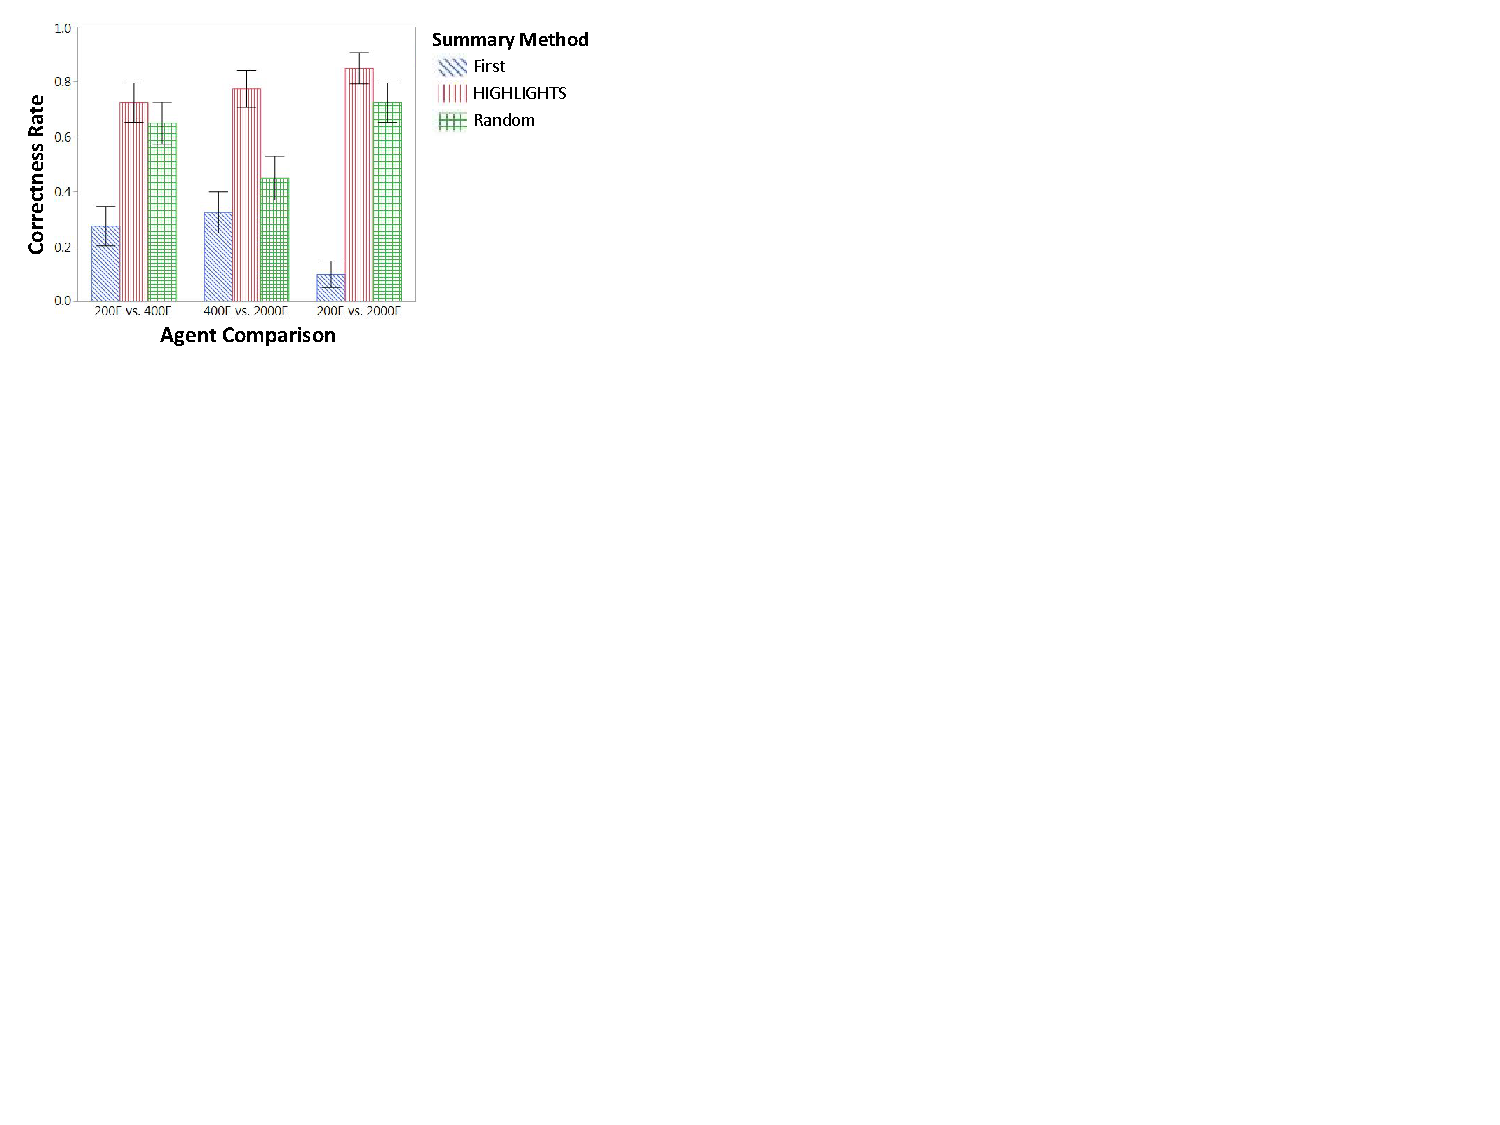
\includegraphics[width=0.9\columnwidth]{figs/correctnessExp1figForPaper.pdf}\\
	\caption{Correctness rate of participants in the agent selection task (Experiment 1).}
	\label{fig:highlightsRes}
	\vspace{-0.3cm}
\end{figure}

Figure~\ref{fig:highlightsConf} shows the distribution of participants' confidence ratings when choosing an agent to play on their behalf. Participants were more confident in their choice of agents when presented with HIGHLIGHTS summaries than they were when presented with summaries generated by \emph{First}. The differences were significant for the medium-difficulty ($\chi^2=22.04, p<0.001, OR = 7.44$) and low-difficulty ($\chi^2=13.84, p<0.001, OR = 3.64$) comparisons. We observed mixed results when comparing participants' confidence when reviewing HIGHLIGHTS and \emph{Random} summaries. When presented with the low-difficulty comparison, participants were significantly more confident when shown \emph{Random} summaries ($\chi^2=6.96, p=0.008, OR = 2.214$)
%, although they performed objectively worse with \emph{Random} summaries, on average (though this difference was not statistically significant). 
When making the low-difficulty comparisons, participants were significantly more confident with HIGHLIGHTS summaries ($\chi^2=5.819, p=0.016, OR = 2.3$). Interestingly, we found no difference in confidence for the medium-difficulty comparison, although participants performed significantly better with HIGHLIGHTS summaries in this agent comparison task. This suggests that people's confidence might not correlate with their actual ability to assess agents' capabilities. We hypothesize that a reason for this is that they only get to review a short summary, and they might think it was sufficient because they are unaware of the information that was \emph{not} included in the summary.
%We also note that as can be seen in Figure~\ref{fig:highlightsConf}, there was much lower variance in participants' confidence ratings for the HIGHLIGHTS summaries compared to the variance in ratings for the two baseline summaries. 



\begin{figure}[h]
	%\centering
	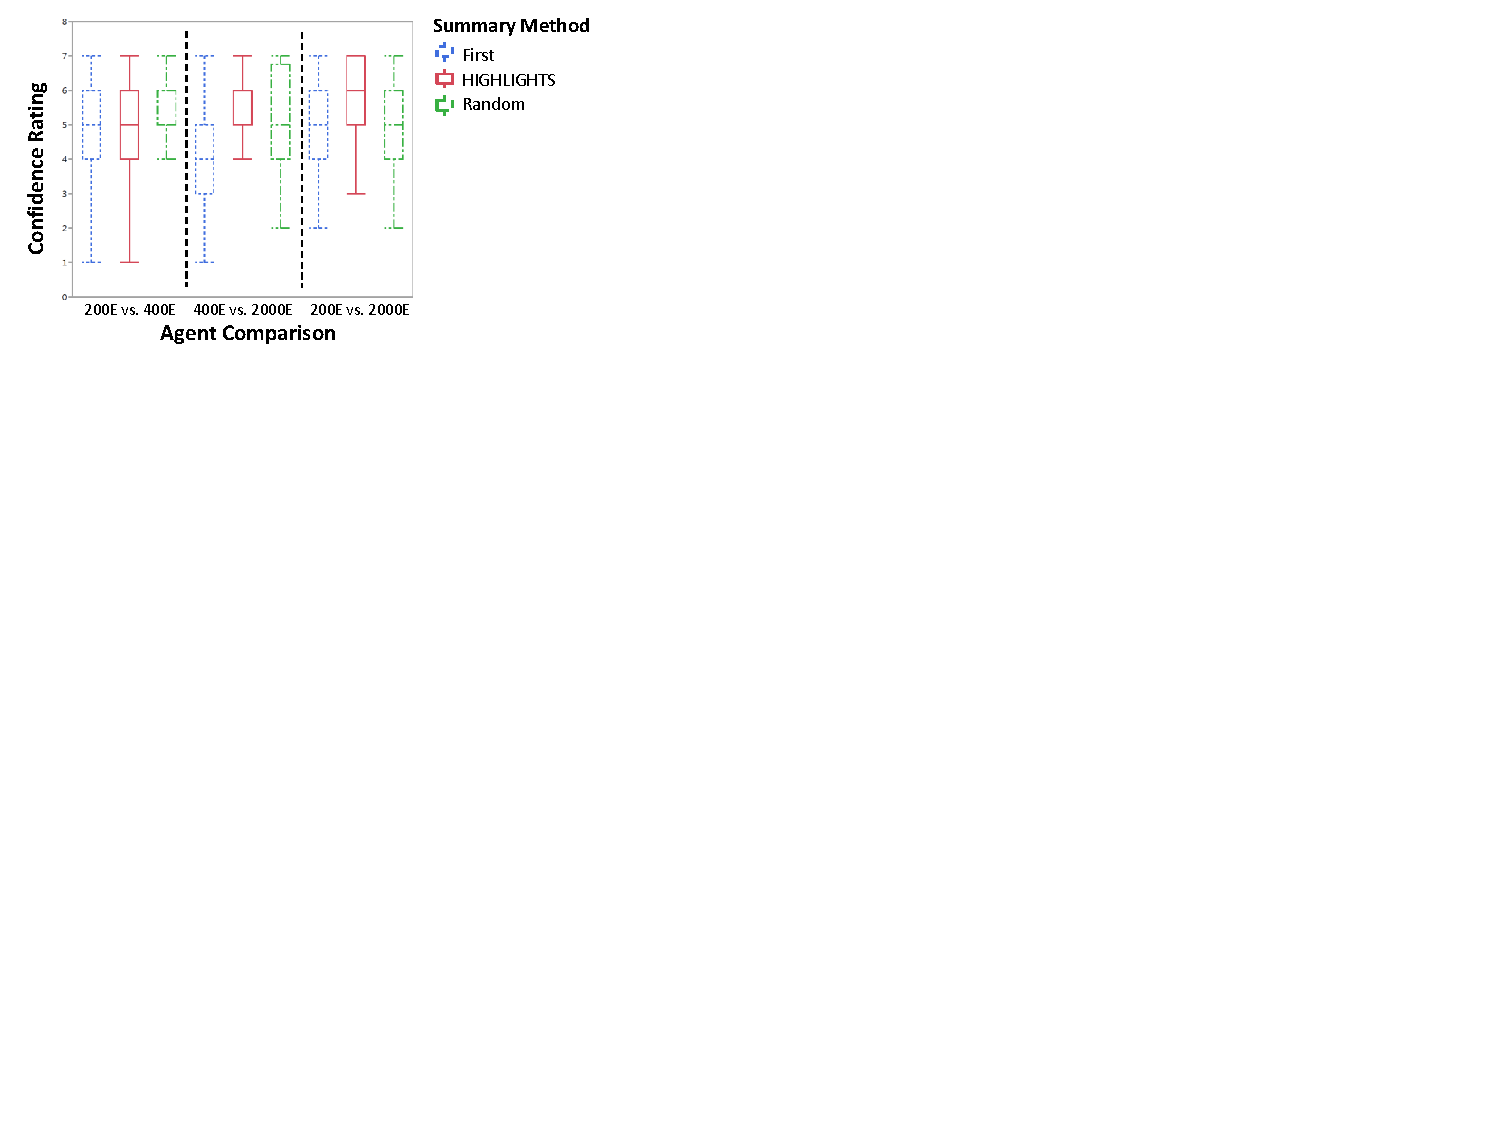
\includegraphics[width=0.89\columnwidth]{figs/confidenceExp1figForPaper.pdf}\\
	\caption{Participants' confidence rating on a scale of 1--7 when selecting an agent (Experiment 1).}
	\label{fig:highlightsConf}
	\vspace{-0.3cm}
\end{figure}


\paragraph{Summary Preferences}
% In addition, we showed participants with pairs of video summaries of \emph{the same} agent, generated by \emph{different} methods and elicited their subjective preference by asking them to rate which summary was more helpful for assessing the capabilities of the agent (they were told the videos were of the same agent). The ratings were on a 1--7 Likert scale where 1 is ``summary A was more helpful'' and 7 is ``summary B was more helpful''. We normalized the scores such that scores closer to 7 suggest a preference for HIGHLIGHTS (in the experiment the assignment to summary A and B was randomized). 
The distribution of participants' subjective preferences ratings for the different summaries are shown in Figure~\ref{fig:highlightsPrefs}. Recall, that a rating closer to 7 means they stated that the summary generated by HIGHLIGHTS was more helpful in assessing the agent's capability, while a rating closer to 1 indicates that they found the other summary (generated by either \emph{First} or \emph{Random}) as more helpful. That is, ratings greater than 4 indicate a preference for HIGHLIGHTS. The ratings are shown separately for each type of agent for which summaries were presented. 

\begin{figure}[h]
	%\centering
	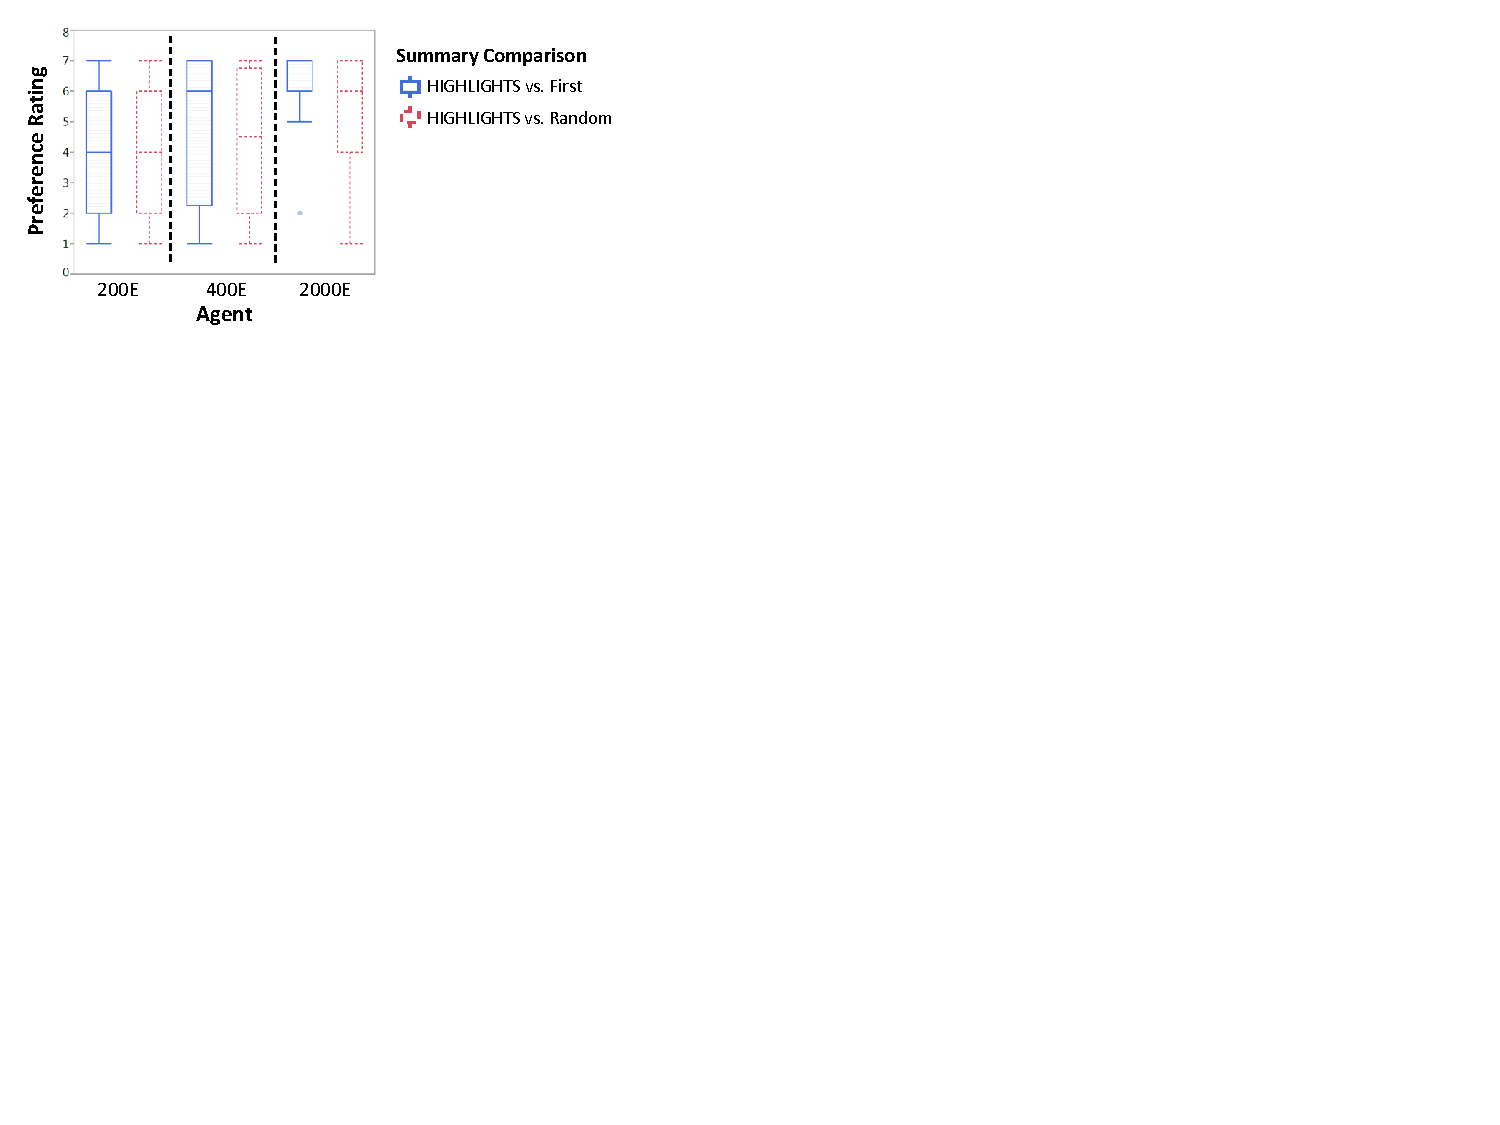
\includegraphics[width=0.85\columnwidth]{figs/preferencesExp1figForPaper.pdf}\\
	\caption{Participants' preference rating on a scale of 1--7, where 7 = ``HIGHLIGHTS is more helpful'' (Experiment 1).}
	\label{fig:highlightsPrefs}
	\vspace{-0.3cm}
\end{figure}

On average, participants preferred summaries generated by HIGHLIGHTS over summaries generated by \emph{First} ($Median = 6$) and summaries generated by \emph{Random} ($Median = 5$). The only statistically significant differences in preferences were for the highest performing agent (\emph{2000E}). The ratings were significantly greater than 4 both when comparing HIGHLIGHTS with \emph{First} ($Median = 7, p<0.001$) and when comparing HIGHLIGHTS with \emph{Random} ($Median = 6, p=0.009$). We attribute this stronger preference to the greater difference between summaries generated by different methods when considering agents that have more capabilities. For example, the highest performing Pacman agent was able to both escape ghosts and eat the power pellets which let it eat ghosts. The HIGHLIGHTS summary for this agent included trajectories demonstrating this capability, while \emph{First} summaries did not show it, and only some \emph{Random} summaries did. Participants often referred to the skills demonstrated in the summary when explaining their ratings of these summaries, e.g. ``A [HIGHLIGHTS] was better for showing how good they were at leading the ghosts.'' In contrast, the lowest performing agent did not have many capabilities, and therefore there was less difference between the summaries generated by the different methods. Another possible explanation for this difference is that because the \emph{200E} and \emph{400E} agents are less trained, their Q-values are less accurate, making their judgment of state importance inferior, and thus potentially making the summaries less useful. 

%When explaining their ratings of the helpfulness of different summaries, participants often referred to the skills demonstrated in the video, e.g. ``A [HIGHLIGHTS] was better for showing how good they were at leading the ghosts'' or the state of the game shown, e.g. ``[video] A shows more of the late game''. Few explanations refereed to the diversity of the summary, e.g. ``[video] A [HIGHLIGHTS] showed more scenarios than B [\emph{First}] did''.





\section{Experiment 2: HIGHLIGHTS-DIV}
Experiment 2 compared summaries generated by the HIGHLIGHTS-DIV algorithm with summaries generated by the basic HIGHLIGHTS algorithm and summaries generated by the \emph{Random} baseline (which significantly outperformed the \emph{First} baseline in Experiment 1). We recruited 48 participants through Amazon Mechanical Turk (25 female, Mean age = 36, STD = 11.6).  

\paragraph{Agent Selection Results} 
Figure~\ref{fig:highlightsDivRes} shows the correctness rates obtained by participants in experiment 2 for each of the summary methods. We begin by comparing HIGHLIGHTS summaries and HIGHLIGHTS-DIV summaries, which is the main focus of this experiment. 
%When analyzing participants' correctness rate for these summaries, we find an interaction effect between the summary method and comparison type, therefore fit a separate model for each comparison type. 
When making the high-difficulty comparison (\emph{200E} vs. \emph{400E} agents), participants were more likely to identify the superior agent when presented with HIGHLIGHTS-DIV summaries ($\chi^2=7.16, p=0.007, OR = 4.2$). We note that participants' performance when presented with HIGHLIGHTS summaries was lower than that of participants in Experiment 1 for the high-difficulty agent comparison. However, since we used a within-subject design, if participants were less attentive, they should also be less successful when presented with HIGHLIGHTS-DIV summaries. The difference between HIGHLIGHTS and HIGHLIGHTS-DIV remains significant even when aggregating the HIGHLIGHTS data from both experiments. We did not find  significant differences for the medium- and low-difficulty agent comparisons. 

When comparing the performance of participants when presented with \emph{Random} summaries with their performance when presented with HIGHLIGHTS or HIGHLIGHTS-DIV summaries, we did not observe an interaction effect between summary and comparison type. Therefore, we fit a single model for each summary comparison (\emph{Random} vs. HIGHLIGHTS and \emph{Random} vs. HIGHLIGHTS-DIV). We found a statistically significant effect for both comparisons, with participants being less successful when presented with \emph{Random} summaries (\emph{Random} vs. HIGHLIGHTS: $\chi^2=20.686, p<0.001, OR = 3.06$; \emph{Random} vs. HIGHLIGHTS-DIV: $\chi^2=27.28, p<0.001, OR = 5.15$). These results reinforce the results of Experiment 1 which showed improved performance with HIGHLIGHTS summaries compared to \emph{Random} summaries. Moreover, while in Experiment 1 we  found a significant difference only for the difficult agent comparison, here we observed significant differences for all agent comparisons.\footnote{It is reasonable to observe different performance levels with \emph{Random} summaries, as different participants could observe different \emph{Random} summaries.} When aggregating the data from both experiments for HIGHLIGHTS and \emph{Random}, we find significant differences for all agent comparisons, strengthening the conclusions from Experiment 1. 

The explanations given by participants for their agent choices were similar to those given by participants in Experiment 1. When making the high-difficulty comparison with the HIGHLIGHTS-DIV summaries, participants often referred to the fact that the summary of the \emph{200E} agent included a trajectory were Pacman was eaten, e.g. ``Player A [200E] gets caught by the ghosts at least once so it looks like Player B [400E] might have the better game'', or to the fact that the \emph{400E} agent was shown eating ghosts, e.g. ``Player B [400E] was able to eat some power pills and blue ghosts to gain more points.'' Explanations for the other comparisons were similar to those given when presented with HIGHLIGHTS summaries described in Section~\ref{sec:exp1res}.

\begin{figure}[h]
	%\centering
	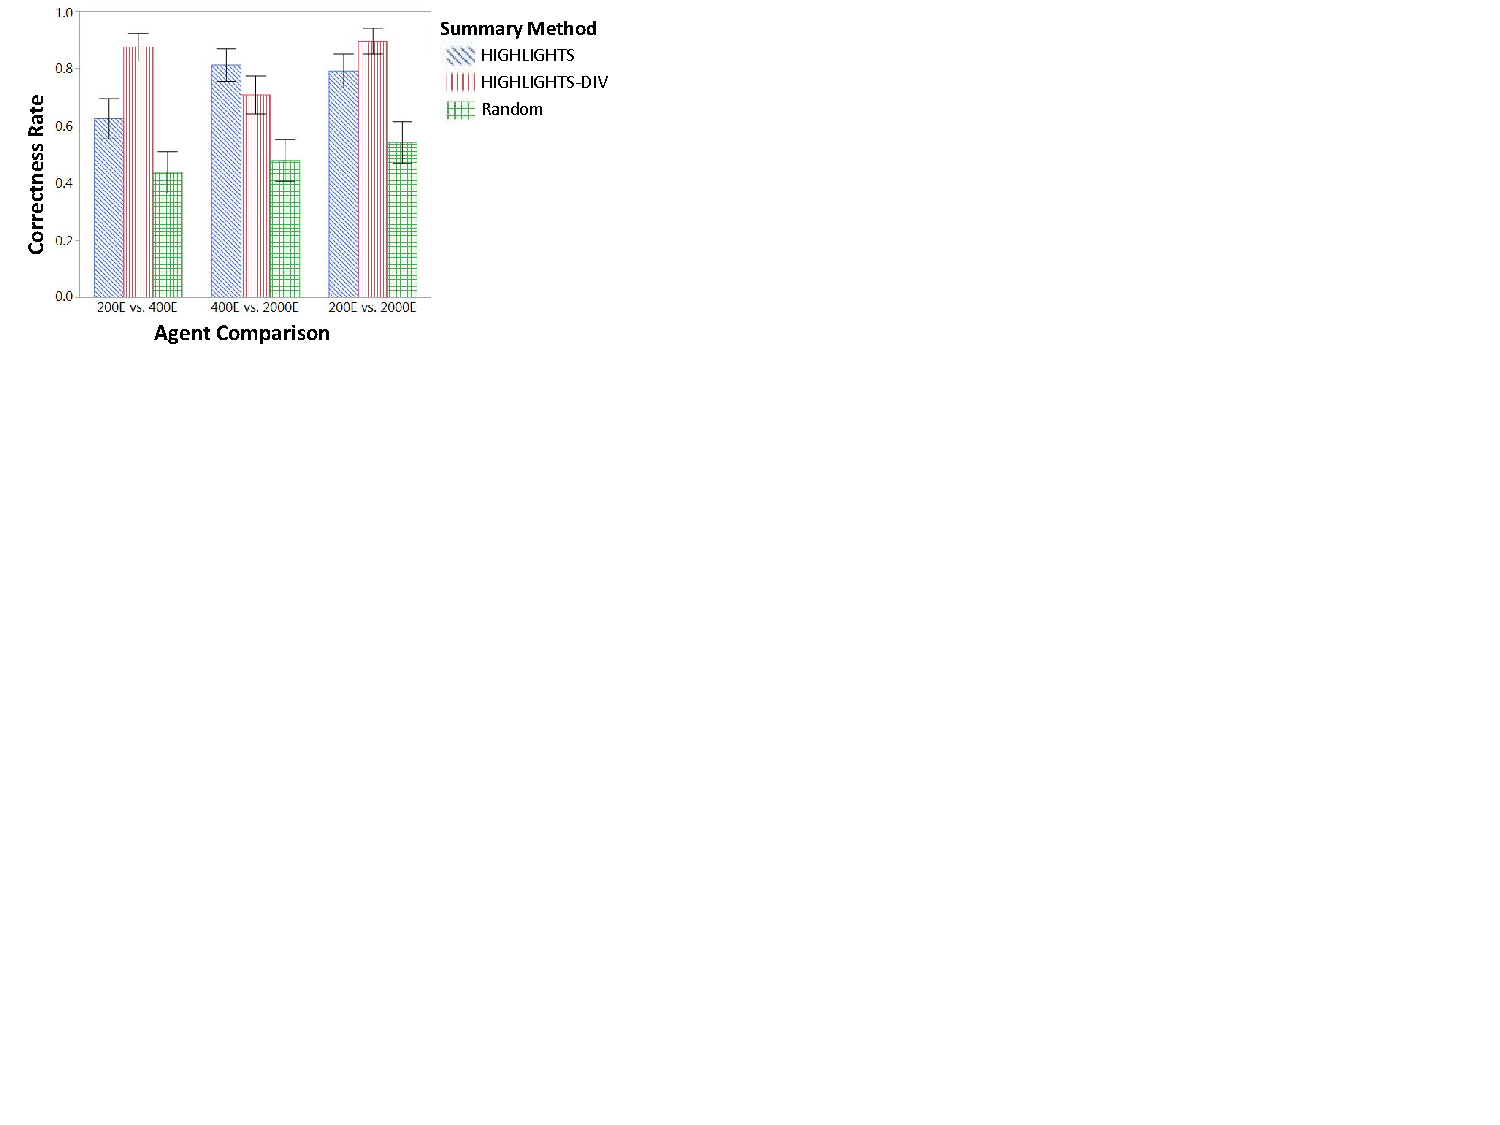
\includegraphics[width=0.9\columnwidth]{figs/correctnessExp2figForPaper.pdf}\\
	\caption{Correctness rate of participants in the agent selection task (Experiment 2).}
	\label{fig:highlightsDivRes}
	\vspace{-0.3cm}
\end{figure}

%The confidence ratings for all summary methods are shown in Figure~\ref{fig:highlightsConfExp2}. 
As in Experiment 1, we observed mixed results in terms of participants' confidence alignment with their actual performance. For the high-difficulty and low-difficulty agent comparisons, Participants' confidence ratings were significantly higher when presented with HIGHLIGHTS-DIV summaries compared to their confidence when reviewing HIGHLIGHTS summaries (high-difficulty: $\chi^2=17.84, p<0.001, OR = 3.68$; low-difficulty: $\chi^2=11.14, p=0.001, OR = 2.82$). We did not observe a statistically significant difference for the medium-difficulty comparison. The higher confidence when shown HIGHLIGHTS-DIV summaries is in line with participants' objective performance for the high-difficulty comparison. We did not find any differences in confidence ratings between HIGHLIGHTS and \emph{Random}, despite the significantly higher objective performance of participants when shown HIGHLIGHTS summaries. When comparing participants' confidence in the HIGHLIGHTS-DIV and \emph{Random} conditions, we found a statistically significant difference for the low-difficulty agent comparison ($\chi^2=16.24, p<0.001, OR = 3.72$). 


% \begin{figure}[h]
% 	%\centering
% 	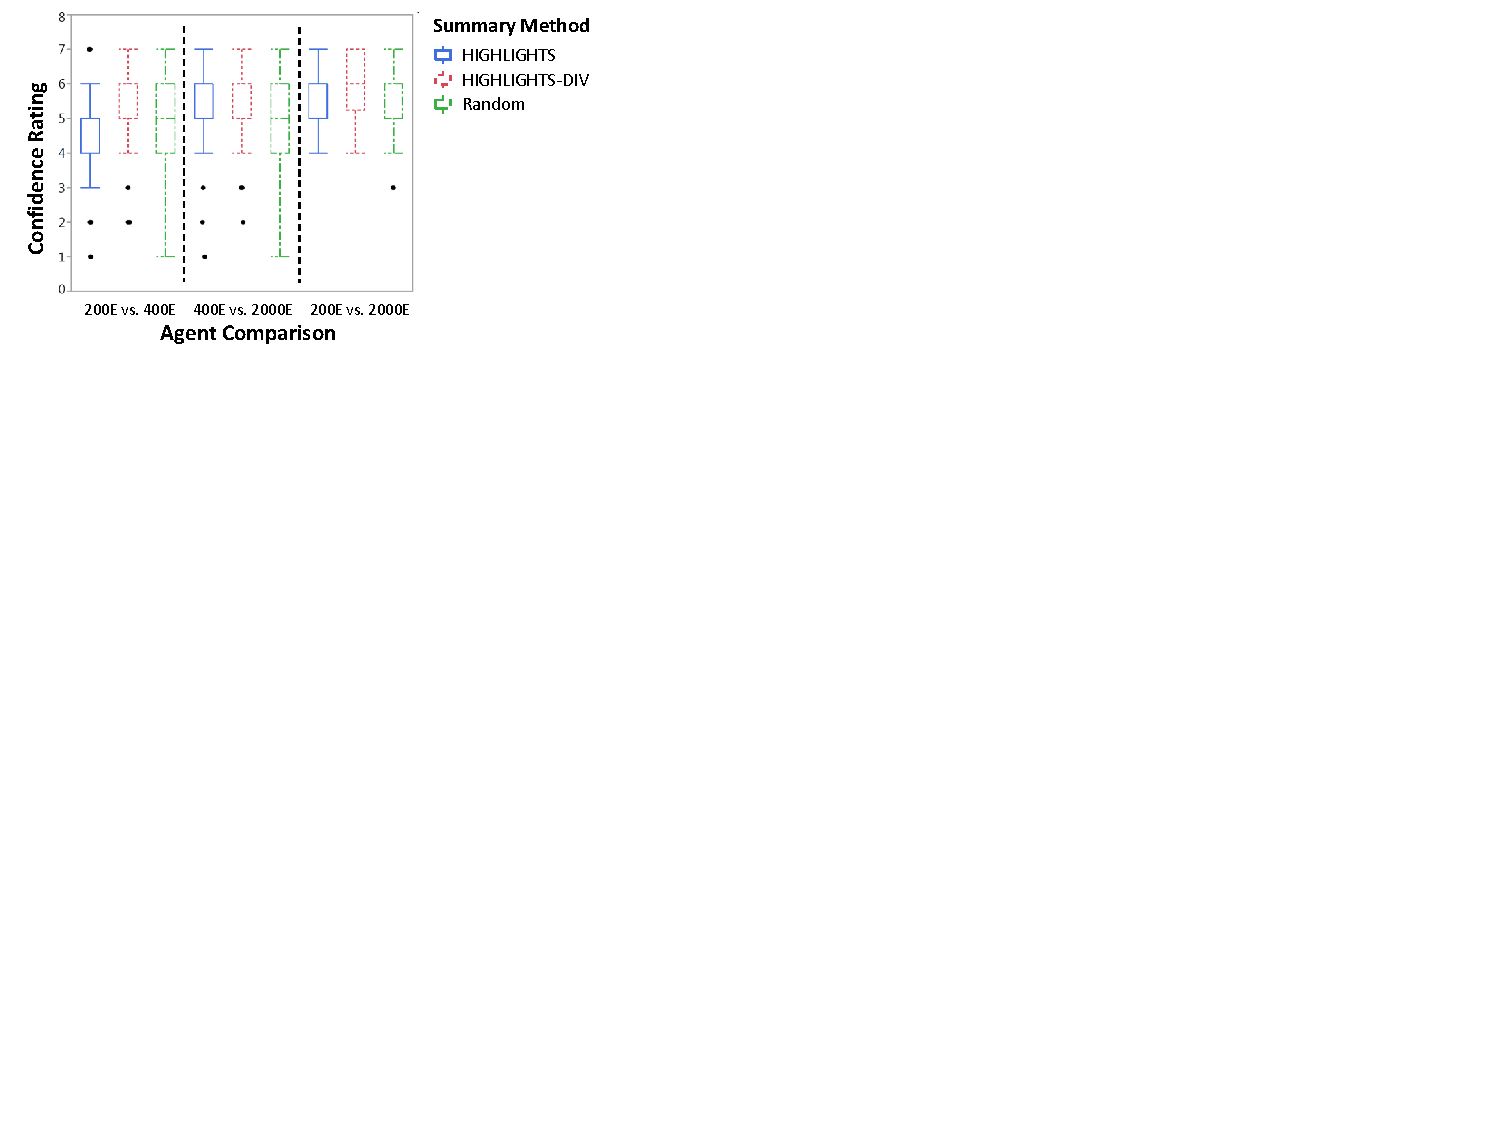
\includegraphics[width=0.85\columnwidth]{figs/confidenceExp2figForPaper.pdf}\\
% 	\caption{Participants' confidence rating on a scale of 1--7 when selecting an agent (Experiment 2).}
% 	\label{fig:highlightsConfExp2}
% 	\vspace{-0.4cm}
% \end{figure}


\paragraph{Summary Preferences}
%Figure~\ref{fig:highlightsPrefsExp2} shows the distribution of participants' preferences ratings.
%\footnote{In Experiment 2 we did not elicit preferences for the \emph{200E} agent summaries to obtain more data for the \emph{400E} and \emph{2000E} agents, for which there were greater differences between different summaries.}
When presented with summaries of the \emph{400E} agent, participants preferred the HIGHLIGHTS-DIV summary over the HIGHLIGHTS summary, though this preference was only marginally significant ($Median = 3, p=0.1$). When explaining their ratings of these summaries participants often referred to skills demonstrated in the summary, e.g. ``The types of explanations provided were similar to those given in Experiment 1 and often referred to the skills demonstrated in the summary, e.g. ``It [HIGLIGHTS-DIV] shows how well the player baited the ghosts and then was able to snack on them.'' We found no difference in preferences between the two summary methods when reviewing summaries of the \emph{2000E} agent  ($Median = 4$). When comparing participants' preferences for HIGHLIGHTS and \emph{Random} summaries, we observed similar results to those obtained in Experiment 1 ($Median = 5$). As in Experiment 1, the difference was significant only when comparing summaries of the \emph{2000E} agent ($Median = 5, p = 0.05$). We did not directly compare HIGHLIGHTS-DIV with \emph{Random} summaries, but the results suggest a preference for HIGHLIGHTS-DIV summaries (as they were preferred over HIGHLIGHTS summaries, which were preferred over \emph{Random} summaries).  
%Participants subjective preferences ratings for summary are shown in Figure~\ref{fig:highlightsPrefs}. Recall, that a rating closer to 7 is means they stated that the summary generated by HIGHLIGHTS was more helpful in assessing the agent's capability, while a rating closer to 1 indicates that they found the other summary (either generated by either \emph{First} or \emph{Random} as more helpful). That is, ratings greater than 4 indicate a preference for HIGHLIGHTS. The ratings are shown separately for each type of agent for which summaries were presented. 

% \begin{figure}[h]
% 	%\centering
% 	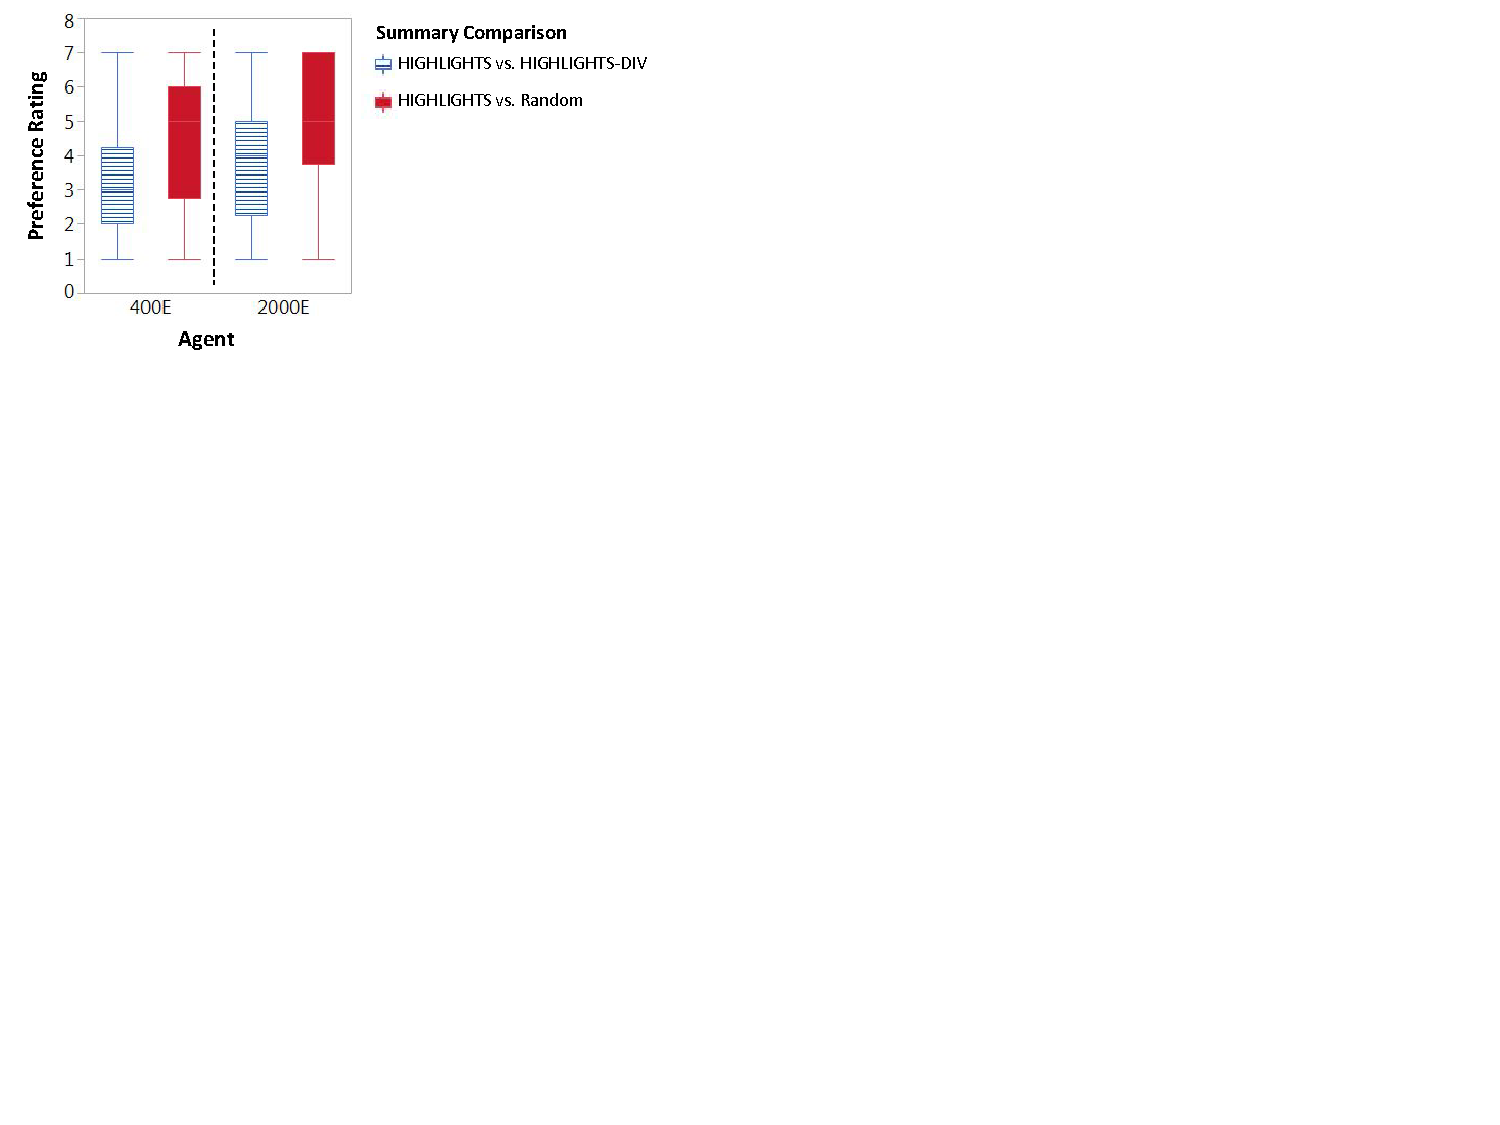
\includegraphics[width=0.8\columnwidth]{figs/preferencesExp2figForPaper.pdf}\\
% 	\caption{Participants' preference rating on a scale of 1--7, where 7 = ``HIGHLIGHTS is more helpful'' (Experiment 2).}
% 	\label{fig:highlightsPrefsExp2}
% 	\vspace{-0.3cm}
% \end{figure}

%On average, participants preferred summaries generated by HIGHLIGHTS over summaries generated by \emph{First} ($Median = 6$) and compared to summaries generated by \emph{Random} ($Median = 5$). The only statistically significant differences were in preferences for HIGHLIGHTS summaries were for the highest performing agent (the ``2000'' agent). The ratings were significantly greater than 4 both when comparing HIGHLIGHTS with \emph{First} ($Median = 7, p<0.001$) and when comparing HIGHLIGHTS with \emph{Random} ($Median = 6, p=0.009$). We attribute this stronger preference to the greater difference between summaries generated by different methods when considering agents that have more capabilities. For example, the highest performing Pacman agent was able to both escape ghosts and eat the power pills which let it eat ghosts. The HIGHLIGHTS summary for this agent included trajectories demonstrating this capability, while \emph{First} summaries did not show it, and only some \emph{Random} summaries did (by chance). This made for a meaningful difference between the summaries. In contrast, the lowest performing agent did not have many capabilities, and therefore there was less difference between the summaries generated by the different methods. 



\section{Discussion \& Future Work}
\label{sec:disc}
With the growing use of intelligent agents, it is important to provide ways for people become more familiar with the the behaviors of such agents, their capabilities and limitations. This paper proposes a new approach for increasing the familiarity of users with agents -- generating summaries of agent behaviors. Our results show that presenting people with ``highlights'' summaries of an agent behavior can help people evaluate the capabilities of different agents. These results provide initial evidence for the potential usefulness of the proposed approach. We next discuss several limitations of the developed HIGHLIGHTS algorithms and possible ways to address them, as well as additional directions for future work. 

%In this work, we  considered two criteria for selecting states to include in the summary: state importance, and the diversity of states. 
The algorithms we described can be improved in several ways. First, the importance measure we used is sensitive to the distribution of Q-values in different states (e.g., it might not make sense in domains where there are many possible actions at any given state, because agents will never consider the worst action). In future work we will define more sophisticated importance measures, e.g., by considering the variance in 
Q-values or regret values. In addition, because the importance assessment was based on the agent's own Q-values, different agents might consider different states as important, and in particular low-quality agents might not be able to recognize states that people will consider important. To mitigate this problem, we will explore ways of assessing importance that do not rely solely on the judgment of the agent itself. For example, aggregating importance values of different agents. In addition, importance could be computed for an entire trajectory rather than for a specific state. Similarly, the diversity of the summary can also be computed based on complete trajectories. We note that while our approach assumed an MDP representation for importance computations, similar notions could also be defined for other decision-making models. For example, with hierarchical plans it might be possible to define a measure that assesses the impact of an action on the ability to achieve a goal.

While considering importance and diversity criteria already improved people's ability to evaluate the performance of different agents compared to the baselines, there are other criteria that should be taken into consideration when generating summaries. For example, in our experiments, participants sometimes referred to specific events when justifying their choice of agents. To ensure that people do not overweight or underweight specific events, the likelihood of encountering states should be reflected in the summary and conveyed to users. In addition, we hypothesize that different summaries may be effective in different contexts. For instance, if the goal of the user is to compare two agents, summaries highlighting states in which their actions differ might be more helpful than summaries that produced for each of the agents separately. Evaluation criteria for summaries can also be extended to include additional metrics such as the ability of people to predict an agent's actions and their ability to collaborate with the agent on a task. 

Our formulation of the summary generation problem assumed a limited budget for the number of trajectories that can be included in the summary. A different way of approaching strategy summarization is framing it as an optimization problem where the goal is to create a minimal summary that satisfies certain criteria (e.g., with respect to coverage of the state space). We will explore such formulations in future work. 

The presentation of summaries is likely to depend on the characteristics of different domains. In the Pacman domain used in our study, presenting a video-clip of the agent was appropriate for conveying the agent's behavior, and showing trajectories that include neighboring states provided people with sufficient context for assessing the agent's actions. This approach could apply more generally to domains where there is a physical agent (e.g., a robot or a self-driving car), but may not be appropriate for some virtual agents (e.g., a personal assistant). In the latter domains, different visualization methods of states will likely be required (e.g., showing some feature-based representation of a state). 

Finally, while automatically generated summaries can provide users with a basic overview of an agent's behavior, in some situations users may require more detailed information, tailored to their needs. To this end, we plan to design collaborative interfaces that let people adjust summaries and explore the behavior of agents in different states. This is particularly important as our experiment showed that people's confidence did not always correlate with the correctness of their assessments, highlighting the importance of providing users with more information about the summaries they observe and more ways to explore them. 




%Our results show that presenting people with ``highlights'' summaries of an agent behavior based on state importance criteria can help them assess the capabilities of different agents, and that considering diversity of trajectories in the summary can further improve these assessments. 

%With the growing use of intelligent agents, it is important to help users understand the capabilities and limitations of such agents. We proposed presenting users with ``highlights'' summaries of agent behaviors to help them gain a better understanding of an agent's global behavior. We 


\begin{acks}
%\textbf{Acknowledgements.} 
We thank Avi Segal, Ken Arnold and Sebastian Gehrmann for their feedback on drafts of this paper.
\end{acks}
%%%%%%%%%%%%%%%%%%%%%%%%%%%%%%%%%%%%%%%%%%%%%%%%%%%%%%%%%%%%%%%%%%%%%%%%%%%%%%%%%%%%%%%%%%%%%%%%%%%%%%%%%
%% bibliography: see CFP for number of permitted pages

\bibliographystyle{ACM-Reference-Format}  % do not change this line!
\balance
\bibliography{lib}  % put name of your .bib file here

\end{document}
